\documentclass[a4paper, 12pt]{article}
\usepackage[a4paper,top=1.5cm, bottom=1.5cm, left=0.5cm, right=1cm]{geometry}
\usepackage[utf8]{inputenc}
\usepackage{mathtext}
\usepackage{amsmath}
\usepackage{amsfonts}
\usepackage{graphicx}
\usepackage{wrapfig}

\usepackage{hyperref}
\usepackage[rgb]{xcolor}
\definecolor{linkcolor}{HTML}{0000FF}												% цвет ссылок
\definecolor{urlcolor}{HTML}{0000FF}												% цвет гиперссылок
\hypersetup{pdfstartview=FitH,  linkcolor=linkcolor,urlcolor=urlcolor, colorlinks=true}
%  Русский язык

\usepackage[T2A]{fontenc}			% кодировка
\usepackage{cmap}



% Математика
\usepackage{amssymb,amsthm} %,mathtools% 
\usepackage[english,russian]{babel}	% локализация и переносы
\usepackage{rotating}
\usepackage{wasysym}
 
\graphicspath{{pictures/}}

\title{\begin{center}Лабораторная работа №1.1.4\end{center}
Измерение интенсивности радиационного фона}
\author{Габорак Александр Витальевич \\ Б02-203}
\date{$30 \ ноября \ 2022 \ г.$}

\begin{document}
    \pagenumbering{gobble}
    \maketitle
    \newpage
    \pagenumbering{arabic}

    \section{Введение}
    \textbf{Цель работы:}
    \begin{itemize}
        \item Применить методы обработки экспериментальных данных для изучения статистических закономерностей при измерении интенсивности радиационного фона
    \end{itemize}

    \vspace{1cm}

    \textbf{В работе используются: }
    \begin{itemize}
        \item счётчик Гейгера-Мюллера
        \item блок питания
        \item компьютер с интерфейсом связи со счётчиком
   \end{itemize}


	\section{Теоретические сведения}
	Регистрация частиц однородна по времени и каждое последующее событие не зависит от предыдущего, поэтому количество отсчетов в одном опыте подчиняются распределению Пуассона, которое при больших числах стремится к нормальному. Стандартная ошибка отдельного измерения через измеренное значение $n$:
	\begin{equation}\label{сигма}
		\sigma=\sqrt{n}
	\end{equation}
	Отсюда следует, что результат измерений с высокой точностью записывается так: 
	\begin{equation}\label{н0}
		n_0=n\pm\sqrt{n}
	\end{equation}
	При $N$ измерениях среднее значение числа частиц за одно измерений равно:
	\begin{equation}\label{нср}
		\overline{n}=\frac{1}{N}\sum_{i=1}^{N} {n_i}
	\end{equation} 
	Стандартную ошибку измерения можно оценить по формуле: 
	\begin{equation}\label{сигмаотд}
		\sigma_{\text{отд}}=\sqrt{\frac{1}{N}\sum_{i=1}^{N}{(n_i-\overline{n})^2}}
	\end{equation}
	Ближе всего к значению $ \sigma_{отд} $ лежит величина $ \sqrt{\overline{n}} $, то есть:
	\begin{equation}
		\label{сигмаотдприб}
		\sigma_{\text{отд}}\thickapprox\sqrt{{\overline{n}}}
	\end{equation}
	Величина $\overline{n}$ не вполне точно совпадает с истинным значением $n_0$ и является случайной. Стандартная ошибка отклонения $\overline{n}$ от $n_0$ может быть определена так:
	\begin{equation}\label{сигманср}
		\sigma_{\overline{n}}=\frac{1}{N}\sqrt{\sum_{i=1}^N{(n_i-\overline{n})^2}}=\frac{\sigma_{\text{отд}}}{\sqrt{N}}
	\end{equation}
	Относительная ошибка отдельного измерения (ожидаемое отличие любого из $n_i$ от $n_0$):
	\begin{equation}
		\varepsilon_{\text{отд}}=\frac{\sigma_{\text{отд}}}{n_i}\thickapprox\frac{1}{\sqrt{n_i}}
	\end{equation}
	Аналогично определяется относительная ошибка среднего по всем измерениям значения $\overline{n}$:
	\begin{equation}\label{эпсилоннср}
		\varepsilon_{\overline{n}}=\frac{\sigma_{\overline{n}}}{\overline{n}}=\frac{\sigma_{\text{отд}}}{\overline{n}\sqrt{N}}\thickapprox\frac{1}{\sqrt{\overline{n}N}}
	\end{equation}
    \newpage
    \section{Ход работы и обработка результатов}
    \paragraph{}
    Проведём измерение, используя интерфейс компьютера. Приведём данные для $20 \ с$, полученные из программы компьютера, в таблицу \ref{20c} и начнём  обработку. Разбивая эти данные по парам и суммируя пары, получим данные для $40 \ с$ (таблица \ref{40c}).
    \paragraph{}
    
    \begin{table}[ht!]
    	\begin{center}
    		\begin{tabular}{|c|c|c|c|c|c|c|c|c|c|c|}
    			\hline
    			$№ \ опыта$ & 1  & 2  & 3  & 4  & 5  & 6  & 7  & 8  & 9  & 10 \\ \hline
    			     0      & 27 & 26 & 29 & 22 & 22 & 26 & 28 & 30 & 19 & 22 \\
    			    10      & 22 & 19 & 26 & 27 & 25 & 31 & 22 & 22 & 29 & 28 \\
    			    20      & 29 & 40 & 34 & 32 & 26 & 29 & 23 & 28 & 16 & 22 \\
    			    30      & 30 & 32 & 22 & 30 & 16 & 28 & 15 & 24 & 25 & 24 \\
    			    40      & 27 & 19 & 25 & 29 & 24 & 24 & 42 & 25 & 28 & 27 \\
    			    50      & 36 & 35 & 28 & 23 & 17 & 27 & 25 & 22 & 25 & 23 \\
    			    60      & 35 & 31 & 29 & 32 & 28 & 37 & 33 & 15 & 22 & 31 \\
    			    70      & 27 & 21 & 31 & 23 & 34 & 30 & 31 & 18 & 22 & 18 \\
    			    80      & 33 & 19 & 27 & 24 & 21 & 34 & 25 & 28 & 18 & 27 \\
    			    90      & 30 & 26 & 37 & 28 & 32 & 24 & 21 & 36 & 30 & 23 \\
    			    100     & 23 & 24 & 21 & 26 & 24 & 24 & 24 & 15 & 30 & 19 \\
    			    110     & 25 & 28 & 25 & 26 & 21 & 24 & 22 & 34 & 29 & 29 \\
    			    120     & 28 & 35 & 31 & 28 & 25 & 26 & 29 & 33 & 24 & 19 \\
    			    130     & 28 & 30 & 27 & 29 & 15 & 32 & 18 & 19 & 24 & 25 \\
    			    140     & 24 & 18 & 32 & 21 & 38 & 26 & 28 & 25 & 33 & 24 \\
    			    150     & 32 & 19 & 22 & 26 & 33 & 28 & 27 & 24 & 27 & 31 \\
    			    160     & 20 & 26 & 27 & 23 & 32 & 23 & 30 & 20 & 25 & 26 \\
    			    170     & 15 & 30 & 38 & 27 & 28 & 26 & 22 & 34 & 22 & 34 \\
    			    180     & 25 & 20 & 25 & 25 & 30 & 26 & 19 & 31 & 17 & 20 \\
    			    190     & 26 & 24 & 27 & 30 & 19 & 25 & 25 & 21 & 26 & 29 \\ \hline
    		\end{tabular}
    		\caption{Число срабатывании счётчика за $20 \ с$} \label{20c}
    	\end{center}
    \end{table}

	\begin{table}[!ht]
		\centering
		\begin{tabular}{|c|c|c|c|c|c|c|c|c|c|c|}
			\hline
			№ опыта & 1  & 2  & 3  & 4  & 5  & 6  & 7  & 8  & 9  & 10 \\ \hline
			   0    & 53 & 51 & 48 & 58 & 41 & 47 & 47 & 48 & 39 & 49 \\
			  10    & 41 & 53 & 56 & 44 & 57 & 53 & 51 & 45 & 56 & 58 \\
			  20    & 69 & 66 & 55 & 51 & 38 & 63 & 59 & 51 & 62 & 43 \\
			  30    & 62 & 52 & 44 & 39 & 49 & 58 & 56 & 47 & 37 & 49 \\
			  40    & 46 & 54 & 48 & 67 & 55 & 42 & 53 & 64 & 53 & 57 \\
			  50    & 71 & 51 & 44 & 47 & 48 & 51 & 48 & 61 & 51 & 58 \\
			  60    & 66 & 61 & 65 & 48 & 53 & 46 & 50 & 55 & 50 & 51 \\
			  70    & 48 & 54 & 64 & 49 & 40 & 45 & 65 & 54 & 56 & 56 \\
			  80    & 52 & 51 & 55 & 53 & 45 & 45 & 50 & 56 & 50 & 37 \\
			  90    & 56 & 65 & 56 & 57 & 53 & 50 & 57 & 44 & 46 & 55 \\ \hline
		\end{tabular}
		\caption{Число срабатывании счётчика за $40 \ с$}
		\label{40c}
	\end{table}

	\newpage
	Проверим связь $\sigma_{отд}\approx \sqrt{\bar{n}}$. Индекс $"1"$ для $20 \ с$ ($ N_1 = 200 $), $"2"$ для $40 \ с$ ($ N_2 = 100 $)
	\[n_{общ} = \sum_i n_i = 5223\]
	\[\bar{n}_1 = \frac{n_{общ}}{N_1} = 26.115\]
	\[\bar{n}_2 = \frac{n_{общ}}{N_2} = 52.230\]
	\[\sigma_{1}=\sqrt{\frac{1}{N_1} \sum_{i=1}^{N_1} (n_i - \bar{n}_i)^2} \approx 5.20\]
	\[\sigma_{2}=\sqrt{\frac{1}{N_2} \sum_{i=1}^{N_2} (n_i - \bar{n}_i)^2} \approx 7.36\]
	\[\sqrt{\bar{n}_1} = 5.11 \approx 5.20 = \sigma_1\]
	\[\sqrt{\bar{n}_2} = 7.23 \approx 7.36 = \sigma_2\]
    Результат эксперимента демонстрирует, что связь между среднеквадратическим отклонением и среднем значении есть $(\sigma \approx \sqrt{\bar{n}})$.
    Теперь определим долю случаев в пределах $\pm\sigma$ и $\pm2\sigma$.

    \begin{table}[ht!]
    \begin{center}
    \begin{tabular}{|c|c|c|c|}
    	\hline
    	\multicolumn{4}{|c|}{$t=20 \ с$}                                                 \\ \hline
    	          Предел           & Число случаев & Доля случаев & Теоретическая оценка \\ \hline
    	 $\pm \sigma_1 = \pm 5.2$  &      142      &     71\%     &         68\%         \\
    	$\pm 2\sigma_1 = \pm 10.4$ &      189      &     95\%     &         95\%         \\ \hline
    	                              \multicolumn{4}{c}{}                               \\ \hline
    	\multicolumn{4}{|c|}{$t=40 \ с$}                                                 \\ \hline
    	          Предел           & Число случаев & Доля случаев & Теоретическая оценка \\ \hline
    	 $\pm \sigma_2 = \pm 7.4$  &      71       &     71\%     &         68\%         \\
    	$\pm 2\sigma_2 = \pm 14.7$ &      95       &     95\%     &         95\%         \\ \hline
    \end{tabular}
    \caption{Количество измерении за пределами $\pm\sigma$ и $\pm2\sigma$} \label{pmsigma}
    \end{center}
    \end{table}

    \paragraph{}
    Из таблицы \ref{pmsigma} следует, что проведённые расчёты с довольно хорошей точностью соответствуют теории. Как видно из графика, относительный разброс данных за $40 \ с$ меньше, чем за $20 \ с$. Подсчитаем, какая разница между этими двумя случаями.
    \[\frac{\sigma_1}{\bar{n}_1} \approx 20\%, \ \ \ \ \frac{\sigma_2}{\bar{n}_2} \approx 14\%\]
    \paragraph{}
    Получаем разницу примерно в 1.4 раза, что и следует от того факта, что $\sigma \approx \sqrt{\bar{n}}$.
    \paragraph{}
    Для финального ответа рассчитаем ошибки средних величин по формулам (\ref{сигманср}) и (\ref{эпсилоннср})
    \[\sigma_{\bar{n}_1} = \frac{\sigma_{1}}{\sqrt{N_1}} \approx 0.37, \ \ \ \  \sigma_{\bar{n}_2} \approx 0.74\]
    \[\varepsilon_{\bar{n}_1} = \frac{\sigma_{\bar{n}_1}}{\bar{n}_1}\approx 1.4\%, \ \ \ \  \varepsilon_{\bar{n}_2}\approx 1.4\%\]
    
    
    Получаем финальный результат
    \[n_{t=20с}=26.12 \pm 0.37\]
    \[n_{t=40с}=52.23 \pm 0.74\]



    \begin{table}[!ht]
    	\centering
    	\begin{tabular}{|l|c|c|c|c|c|c|c|}
    		\hline
    		Число импульсов $n_i$ &  15   &  16  &  17   &  18   &  19   &  20  &  21   \\ \hline
    		Число случаев         &   5   &  2   &   2   &   5   &  10   &  4   &   7   \\ \hline
    		Доля случаев $w_n$    & 0.025 & 0.01 & 0.01  & 0.025 & 0.05  & 0.02 & 0.035 \\ \hline\hline
    		Число импульсов $n_i$ &  22   &  23  &  24   &  25   &  26   &  27  &  28   \\ \hline
    		Число случаев         &  15   &  8   &  17   &  18   &  16   &  14  &  16   \\ \hline
    		Доля случаев $w_n$    & 0.075 & 0.04 & 0.085 & 0.09  & 0.08  & 0.07 & 0.08  \\ \hline\hline
    		Число импульсов $n_i$ &  29   &  30  &  31   &  32   &  33   &  34  &  35   \\ \hline
    		Число случаев         &  11   &  12  &   8   &   8   &   5   &  6   &   3   \\ \hline
    		Доля случаев $w_n$    & 0.055 & 0.06 & 0.04  & 0.04  & 0.025 & 0.03 & 0.015 \\ \hline\hline
    		Число импульсов $n_i$ &  36   &  37  &  38   &  39   &  40   &  41  &  42   \\ \hline
    		Число случаев         &   2   &  2   &   2   &   0   &   1   &  0   &   1   \\ \hline
    		Доля случаев $w_n$    & 0.01  & 0.01 & 0.01  &   0   & 0.005 &  0   & 0.005 \\ \hline
    	\end{tabular}
    	\caption{Данные для гистограммы за $20 \ с$}
    	\label{gist20 }
    \end{table}
    \newpage

    \begin{table}[!ht]
    	\centering
    	\begin{tabular}{|l|c|c|c|c|c|c|c|}
    		\hline
    		Число импульсов $n_i$ &  37  &  38  &  39  &  40  &  41  &  42  &  43    \\ \hline
    		Число случаев         &  2   &  1   &  2   &  1   &  2   &  1   &  1     \\ \hline
    		Доля случаев $w_n$    & 0.02 & 0.01 & 0.02 & 0.01 & 0.02 & 0.01 & 0.01   \\ \hline\hline
    		Число импульсов $n_i$ &  44  &  45  &  46  &  47  &  48  &  49  &  50    \\ \hline
    		Число случаев         &  4   &  4   &  3   &  4   &  7   &  4   &  5     \\ \hline
    		Доля случаев $w_n$    & 0.04 & 0.04 & 0.03 & 0.04 & 0.07 & 0.04 & 0.05   \\ \hline\hline
    		Число импульсов $n_i$ &  51  &  52  &  53  &  54  &  55  &  56  &  57    \\ \hline
    		Число случаев         &  9   &  2   &  8   &  3   &  5   &  8   &  4     \\ \hline
    		Доля случаев $w_n$    & 0.09 & 0.02 & 0.08 & 0.03 & 0.05 & 0.08 & 0.04   \\ \hline\hline
    		Число импульсов $n_i$ &  58  &  59  &  60  &  61  &  62  &  63  &  64    \\ \hline
    		Число случаев         &  4   &  1   &  0   &  2   &  2   &  1   &  2     \\ \hline
    		Доля случаев $w_n$    & 0.04 & 0.01 &  0   & 0.02 & 0.02 & 0.01 & 0.02   \\ \hline\hline
    		Число импульсов $n_i$ &  65  &  66  &  67  &  68  &  69  &  70  &  71    \\ \hline
    		Число случаев         &  3   &  2   &  1   &  0   &  1   &  0   &  1     \\ \hline
    		Доля случаев $w_n$    & 0.03 & 0.02 & 0.01 &  0   & 0.01 &  0   & 0.01   \\ \hline
    	\end{tabular}
    	\caption{Данные для гистограммы за $40 \ с$}
    	\label{gist40 }
    \end{table}

    \newpage

    \begin{sidewaysfigure}
        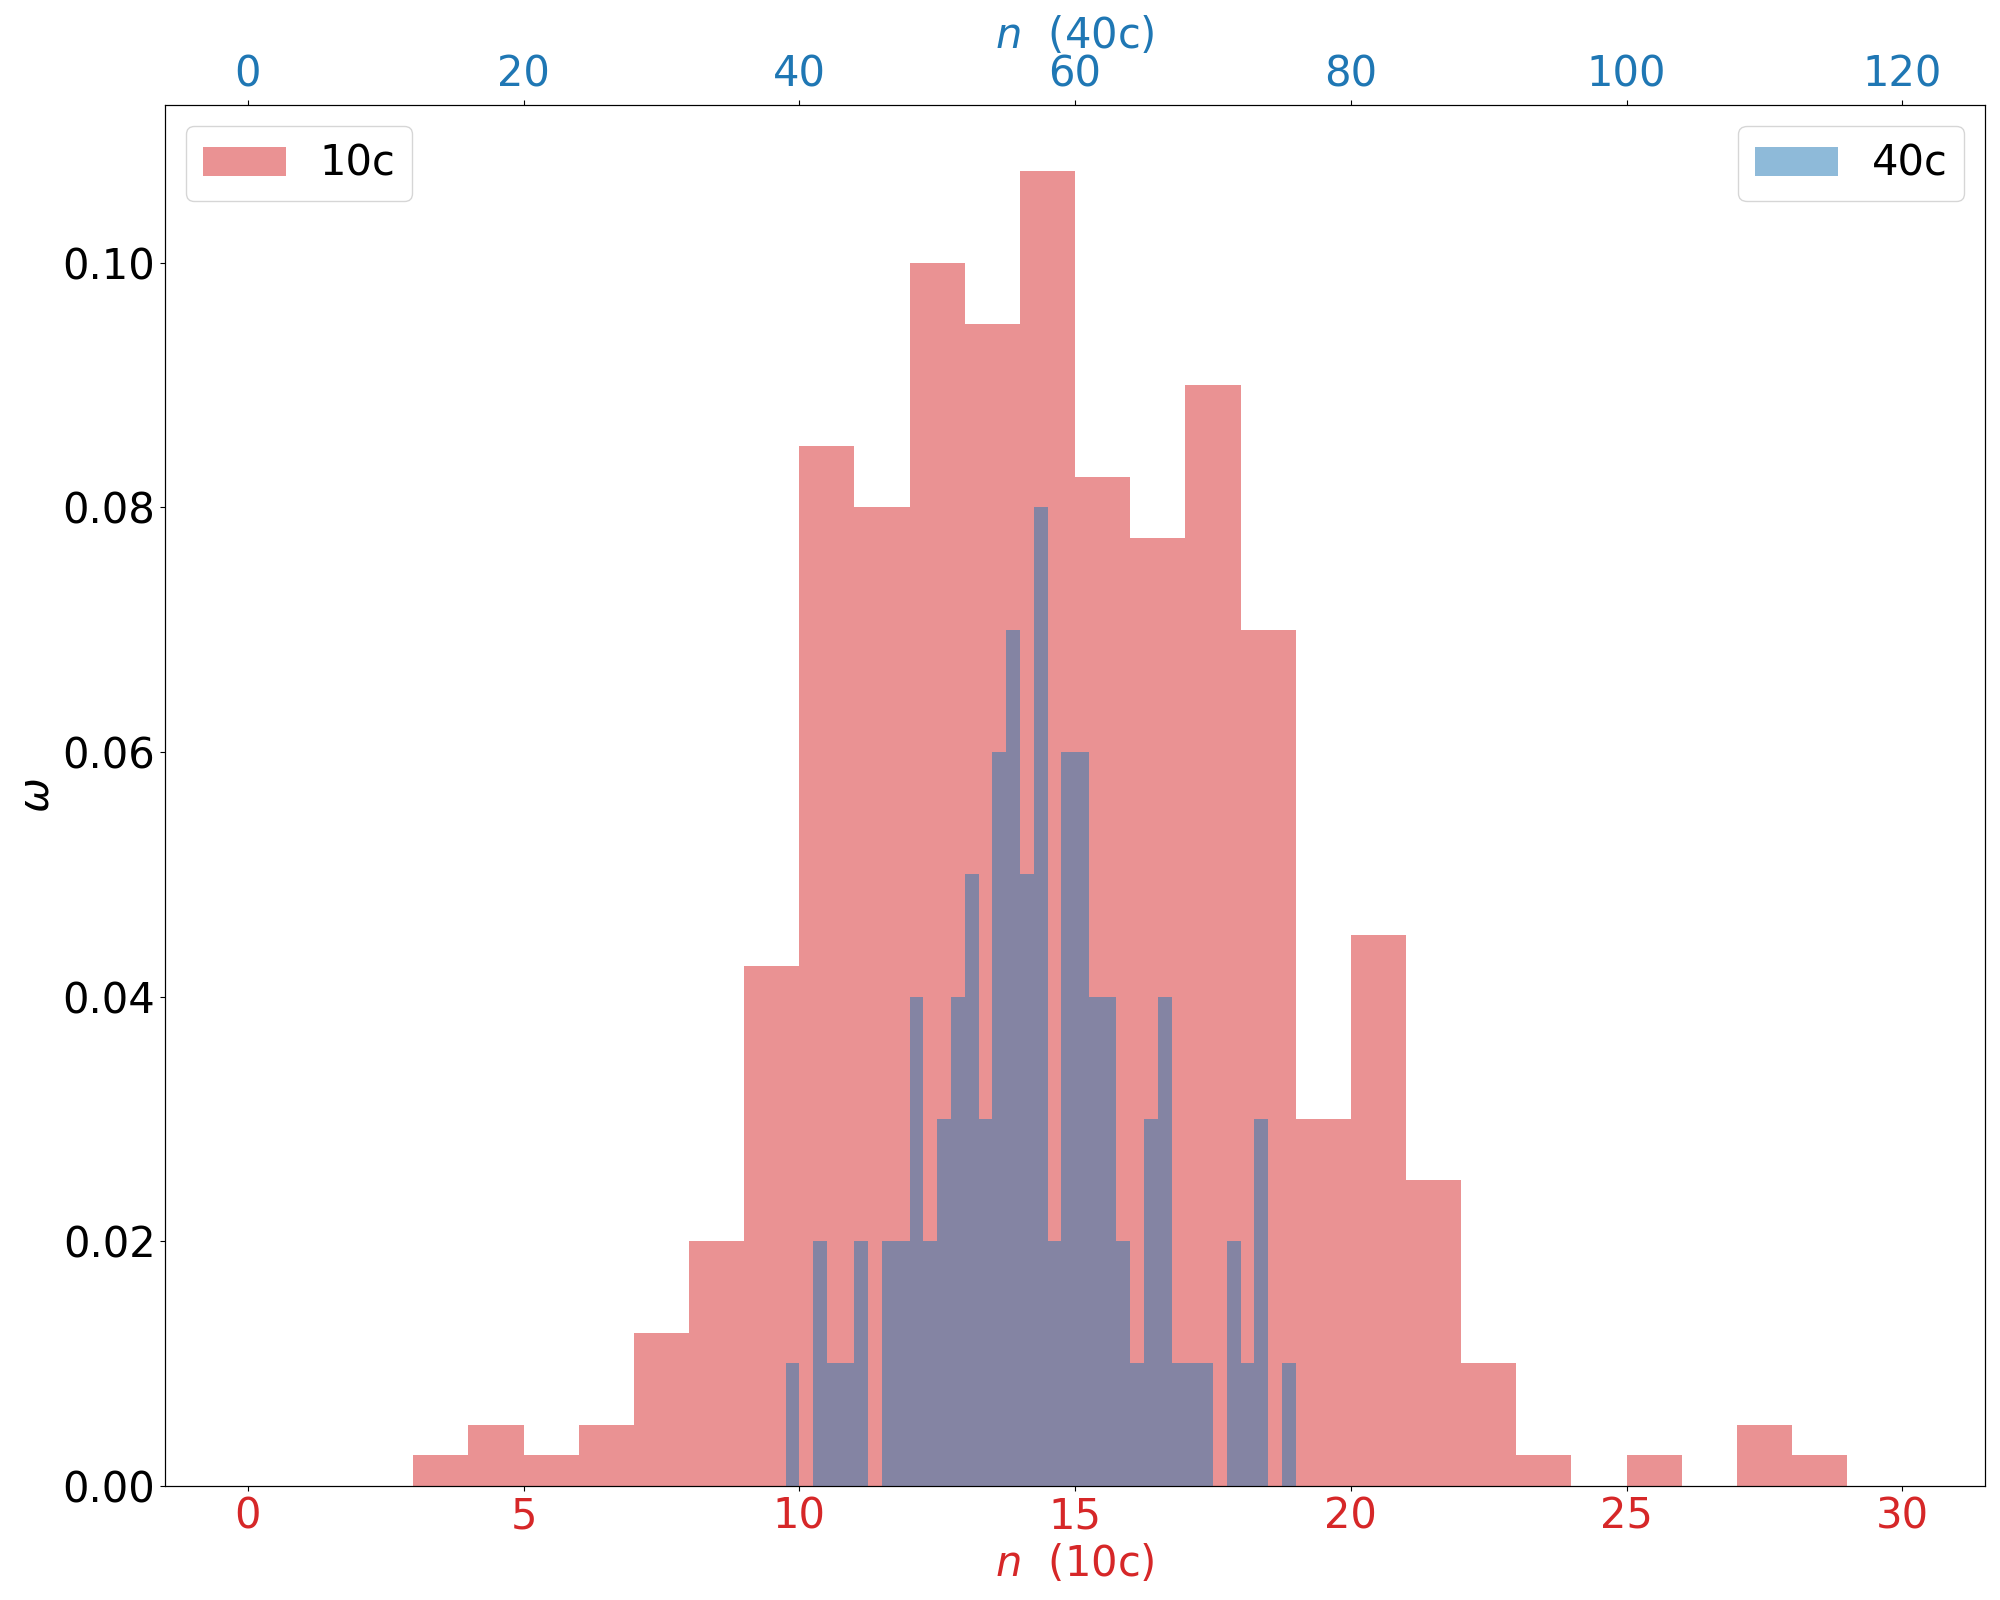
\includegraphics[scale=0.45]{histogram.png}
        \caption{Гистограммы для $t=20 \ с$ и $t=40 \ с$}
    \end{sidewaysfigure}
\end{document}
